\documentclass[a4paper,twoside]{memoir}
% Set up encoding

\usepackage{graphicx,color}
\definecolor{black}{rgb}{0,0,0}
\makeatletter
\newlength{\numberheight}
\makechapterstyle{TroelsPedersen}{%
\setlength{\beforechapskip}{-20pt}
\setlength{\midchapskip}{0pt}
\setlength{\afterchapskip}{40pt}
\renewcommand{\chapnamefont}{\normalfont\LARGE\itshape}
\renewcommand{\chapnumfont}{\normalfont\HUGE\itshape\color{black}}
\renewcommand{\chaptitlefont}{\normalfont\HUGE\itshape\color{black}}
\renewcommand{\afterchapternum}{}
\renewcommand{\printchaptername}{}
\setlength{\numberheight}{20mm}
\renewcommand{\chapternamenum}{}%
\renewcommand{\printchapternum}{%
\sidebar{\makebox[0pt][l]{%
\resizebox{!}{\numberheight}{\chapnumfont\thechapter}}}}%
\renewcommand\printchaptertitle[1]{\chaptitlefont##1}
}
\makeatother
\chapterstyle{TroelsPedersen}

\usepackage[utf8]{inputenc}

% Mulighed for at definere acronyms
\usepackage{acronym}

%package for linenumbers
\usepackage{lineno} 

% Load up bibliography.
\usepackage[authoryear]{natbib}
\setcitestyle{numbers,square}
% Bibliography style.
\bibliographystyle{plainnat}

% Algorithm support.
\usepackage{algorithmic}
\usepackage{algorithm}
\usepackage{subfig}
\usepackage{amsmath}
\usepackage{amsfonts}
% Make algorithms appear as procedures instead.
\floatname{algorithm}{Procedure}
\renewcommand{\algorithmicrequire}{\textbf{Input:}}
\renewcommand{\algorithmicensure}{\textbf{Output:}}

% Image frames.
\setlength{\fboxsep}{0pt}
\setlength{\fboxrule}{0.5pt}

% Also, images.
\usepackage{graphicx}

% tabeller der strækker sig over flere sider
\usepackage{longtable}

% flere tabel-muligheder
\usepackage{multirow}

% bedre enumerate
\usepackage{enumitem}

% Mulighed for if-then-else sætning!
\usepackage{ifthen}

% Todo notes here and there.
% write instead for disable: \usepackage[disable]{todonotes}
\usepackage{todonotes}

% Forbedrede floats.
\usepackage{float}
\usepackage{rotating}

\newsubfloat{figure}

% Special symbols availability.
\usepackage{amssymb}

% Email @
\usepackage{marvosym}

%Degree symbol
\usepackage{gensymb}

% Wrap figure
\usepackage{wrapfig}

% Remove subsection numbering
\renewcommand{\thesubsection}{}
\makeatletter
\def\@seccntformat#1{\csname #1ignore\expandafter\endcsname\csname the#1\endcsname\quad}
\let\subsectionignore\@gobbletwo
\let\latex@numberline\numberline
\def\numberline#1{\if\relax#1\relax\else\latex@numberline{#1}\fi}
\makeatother

%landscape mode
\usepackage{lscape}

\usepackage{booktabs}
\usepackage{hvfloat}
\usepackage{units}

%Fun with captions
\usepackage{caption}


% Neat-o referencer...o.
\usepackage{bookmark,hyperref}
\usepackage{nameref}

\newcommand{\secref}[1]{Section \ref{#1}}
\newcommand{\chapref}[1]{Chapter \ref{#1}}
\newcommand{\appref}[1]{Appendix \ref{#1}}

% Skriver Appendix foran Appendices
\renewcommand*{\cftpartname}{PART~}
%\renewcommand*{\cftchaptername}{\chaptername~}
\renewcommand*{\cftappendixname}{\appendixname~}
%\renewcommand*{\cftchapteraftersnum}{.}% dot after the number
%\setlength{\cftchapternumwidth}{2em}

% Operationel semantik
\newcommand{\lag}{\langle}
\newcommand{\rag}{\rangle}
\newcommand{\setof}[2]{\ensuremath{\{ #1 \mid #2 \}}}
\newcommand{\set}[1]{\ensuremath{\{ #1 \}}}
\newcommand{\besk}[1]{\ensuremath{\lag #1 \rag}}
\newcommand{\ra}{\rightarrow}
\newcommand{\lra}{\longrightarrow}
\newcommand{\Ra}{\Rightarrow}

% CODE %
\usepackage{listings}
\usepackage{color}
%\usepackage{bera}
\definecolor{gray}{rgb}{0.4,0.4,0.4}
\definecolor{darkblue}{rgb}{0.0,0.0,0.6}
\definecolor{cyan}{rgb}{0.0,0.6,0.6}
\definecolor{dkgreen}{rgb}{0,.6,0}
\definecolor{dkblue}{rgb}{0,0,.6}
\definecolor{dkyellow}{cmyk}{0,0,.8,.3}

\lstset{
  basicstyle=\ttfamily,
  columns=fullflexible,
  showstringspaces=false,
  commentstyle=\color{gray}\upshape,
  basicstyle=\small,
  numberstyle=\footnotesize,
  numbers=left,
  captionpos=b,
  stepnumber=1,
  numbersep=10pt,
  tabsize=4,
  breaklines=true,
  literate=
  {æ}{{\ae}}1
  {Æ}{{\AE}}1
  {ø}{{\o}}1
  {Ø}{{\O}}1
  {å}{{\r{a}}}1
  {Å}{{\r{A}}}1
  {§}{{\S}}1
  {é}{{\'{e}}}1
}
% Define markup of XML
\lstdefinelanguage{XML}
{
  morestring=[b]",
  morestring=[s]{>}{<},
  morecomment=[s]{<?}{?>},
  identifierstyle=\color{darkblue},
  keywordstyle=\color{cyan},
  morekeywords={id, target, type, category, value, point, correct, rows, width, time}% list your attributes here
}
% Define markup of C#
\lstdefinelanguage{CSharp}[Visual]{C++}
{
	identifierstyle=\color{darkblue},
	commentstyle=\color{green!70!black}\itshape ,
	stringstyle=\color{gray},
	sensitive=true,
	morestring=[b]",
	morestring=[b]',
	morecomment=[l]//,
	morecomment=[n]{/*}{*/}
}

% Define markup of Javascript
\lstdefinelanguage{JavaScript}{
  keywords={typeof, new, true, false, catch, function, return, null, catch, switch, var, if, in, while, do, else, case, break},
  keywordstyle=\color{blue}\bfseries,
  ndkeywords={class, export, boolean, throw, implements, import, this},
  ndkeywordstyle=\color{darkgray}\bfseries,
  identifierstyle=\color{black},
  sensitive=false,
  comment=[l]{//},
  morecomment=[s]{/*}{*/},
  commentstyle=\color{purple}\ttfamily,
  stringstyle=\color{red}\ttfamily,
  morestring=[b]',
  morestring=[b]"
}

% Define markup of Java
\definecolor{dkgreen}{rgb}{0,0.6,0}
\definecolor{gray}{rgb}{0.5,0.5,0.5}
\definecolor{mauve}{rgb}{0.58,0,0.82}
\definecolor{keywordpurple}{RGB}{145, 0, 109}
\definecolor{background}{RGB}{240, 240, 240}
 
\lstset{
  language=java,
  %basicstyle=\footnotesize,       % the size of the fonts that are used for the code
  numbers=left,                   % where to put the line-numbers
  numberstyle=\tiny\color{black},  % the style that is used for the line-numbers
  stepnumber=1,                   % the step between two line-numbers. If it's 1, each line will be numbered 
  numbersep=5pt,                  % how far the line-numbers are from the code
  backgroundcolor=\color{background},  % choose the background color. You must add \usepackage{color}
  showspaces=false,               % show spaces adding particular underscores
  showstringspaces=false,         % underline spaces within strings
  showtabs=false,                 % show tabs within strings adding particular underscores
  frame=single,                   % adds a frame around the code
  rulecolor=\color{black},        % if not set, the frame-color may be changed on line-breaks within not-black text (e.g. comments (green here))
  tabsize=4,                      % sets default tabsize to 4 spaces
  captionpos=b,                   % sets the caption-position to bottom
  breaklines=true,                % sets automatic line breaking
  breakatwhitespace=false,        % sets if automatic breaks should only happen at whitespace
  title=\lstname,                 % show the filename of files included with \lstinputlisting;
                                  % also try caption instead of title
  keywordstyle=\color{keywordpurple}\bfseries,      % keyword style
  commentstyle=\color{dkgreen},   % comment style
  stringstyle=\color{blue},      % string literal style
  escapeinside={\%*}{*)},         % if you want to add a comment within your code
  morekeywords={*,...},           % if you want to add more keywords to the set
  morecomment=[l]//               % set // to register as a comment (for a line)
}

% Define markup of JSON
\colorlet{punct}{red!60!black}
\colorlet{delim}{red!60!black}
\colorlet{numb}{magenta!60!black}
\lstdefinelanguage{json}{
    basicstyle=\footnotesize,
    numbers=left,
    numberstyle=\tiny\color{black},
    identifierstyle=\color{dkgreen},
    stepnumber=1,
    numbersep=5pt,
    showspaces=false,
    showstringspaces=false,
    showtabs=false,
    breaklines=true,
    breakatwhitespace=false,
    tabsize=4,
    rulecolor=\color{black},
    captionpos=b,
    title=\lstname,
    frame=single,
    backgroundcolor=\color{background},
    literate=
     *{0}{{{\color{numb}0}}}{1}
      {1}{{{\color{numb}1}}}{1}
      {2}{{{\color{numb}2}}}{1}
      {3}{{{\color{numb}3}}}{1}
      {4}{{{\color{numb}4}}}{1}
      {5}{{{\color{numb}5}}}{1}
      {6}{{{\color{numb}6}}}{1}
      {7}{{{\color{numb}7}}}{1}
      {8}{{{\color{numb}8}}}{1}
      {9}{{{\color{numb}9}}}{1}
      {:}{{{\color{punct}{:}}}}{1}
      {,}{{{\color{punct}{,}}}}{1}
      {\{}{{{\color{delim}{\{}}}}{1}
      {\}}{{{\color{delim}{\}}}}}{1}
      {[}{{{\color{delim}{[}}}}{1}
      {]}{{{\color{delim}{]}}}}{1},
}

% pretty inline med background highlight
\newcommand{\inline}[1]{\colorbox{background}{\lstinline|#1|}}

\lstdefinelanguage{phpstyle}{
  language        = php,
  keywordstyle    = \color{dkblue},
  morekeywords    = {function, return, public},
  stringstyle     = \color{red}
  }

\lstdefinelanguage{KAPAOOW}{
 sensitive=false,
 keywords={character, characters, action, end, if, then, else, from, to, downto, next, while, loop, use, turn, begins, ends, select, wins, draw, random, of, case, cases, enemy, player, start, skip, attack, types, damage, defend, by, using, message, and, or, is, value, mod},
 identifierstyle=\itshape,
 keywordstyle=\bfseries,
 stringstyle=\normalfont,
 morestring=[b]",
 comment=[l]{//},
 commentstyle=\color{gray}
}

% hack fra nettet.
% http://tex.stackexchange.com/questions/1230/reference-name-of-description-list-item-in-latex
\makeatletter
\let\orgdescriptionlabel\descriptionlabel
\renewcommand*{\descriptionlabel}[1]{
  \let\orglabel\label
  \let\label\@gobble
  \phantomsection
  \edef\@currentlabel{#1}
  %\edef\@currentlabelname{#1}
%  \let\label\orglabel
  \orgdescriptionlabel{#1}
}
\makeatother
% Rettehak. Meget lettere end \checkmark
\newcommand{\yes}{\checkmark}


% Create a new command, HRule, to insert some nice horisontal rules on the title page.
\newcommand{\HRule}{\rule{\linewidth}{0.3mm}}

% New command for two figures, side by side.
\newcommand{\twofigs}[6]
{
	\begin{figure}[H]
		\begin{minipage}[t]{0.5\columnwidth}
		\centering
		\includegraphics[width=0.8\columnwidth]{img/#1}
		\caption{#2\label{#3}}
		\end{minipage}
		\hspace{0.5cm}
		\begin{minipage}[t]{0.5\columnwidth}
		\centering
		\includegraphics[width=0.8\columnwidth]{img/#4}
		\caption{#5\label{#6}}
		\end{minipage}
	\end{figure}
}

% Sørg for at paragrafplads ikke spildes.
\raggedbottom

% Package til at regne forskellen ud mellem 2 labels
\usepackage{refcount}
\newcommand{\pagedifference}[2]{\number\numexpr\getpagerefnumber{#2}+1-\getpagerefnumber{#1}\relax}


% Fancy chapter style


\usepackage{lipsum}

%Laver fancy ting her. Noget med at overwrite noget includegraphics for at kunne bruge commands som parameter til den
\makeatletter
\protected\def\includeGraphics{\@testopt\roy@includegraphics{}}
\def\roy@includegraphics[#1]#2{%
  \begingroup
  % Every expandable token in #1 may be expanded here:
  \edef\x{\endgroup\noexpand\includegraphics[#1]}\x{#2}%
}
\makeatother

\newcommand{\theAngle}{90} %vinkel brugt til at rotere med, bliver renewed i \landscapefigure

%Indsætter figure i landscape og roterer billedet efter om det er højre eller venstre side
\newcommand{\landscapefigure}[4]
{
\ifthenelse{\isodd{\thepage}}
{% ulige sidetal = højre side
\renewcommand{\theAngle}{90}
}
{% lige sidetal = venstre side
\renewcommand{\theAngle}{270}
}

\begin{figure}[H]
\centering
\includegraphics[angle=\theAngle ,#1]{img/#2}
\caption{#3}
\label{#4}
\end{figure}
}

\hyphenation{guard-i-an}


\title{Software Innovation: Miniproject}
\author{Jacob Karsten Wortmann\\Jesper Riemer Andersen\\Nicklas Andersen\\Sam Sepstrup Olesen\\Simon Reedtz Olesen}

\begin{document}
\maketitle

\subsection*{Brief description}
The idea of the project is to make an interactive cookbook on the android platform that can give you suggestions of recipes based on chosen ingredients. An advantage of the interactive recipe search based on ingredients could be that whenever you find an interesting ingredient in the store, you can choose this ingredient in the application and quickly get relevant suggestions of recipes and thereby identify which additional ingredients you need to buy. Another use for this functionality is to find interesting recipes that you can make with the ingredients you already have at home or few additional ingredients.

\subsection*{Challenges}
The main challenge of the project is to make an efficient search algorithm that rivals the other similar applications on the market. The problem with the other existing solutions is that if you for example input ``eggs'' and ``chicken'', you will get many different recipes of how to prepare eggs, and not on how to combine the two ingredients. The overall design of the application can also prove to be a major challenge because we have to fit a large amount of information on a relatively small mobile screen.

%\section*{Section 1}
% a brief description of your initial project idea at the start of the semester (no more than half a page).

\subsection*{Problem Domain}

When a user stands in their kitchen or in the supermarket and wants to look up recipes for dinner, they must be able to access those easily.

Our application focuses on making it easy to access recipes on mobile devices. We want to split up the recipes in core and optional ingredients, in order to optimise the search results the user gets. For this we need to analyse each recipe that will be used in the application.

\subsection*{Use Context}

The application can be used in different scenarios, for example the user can be at home and type in the items they have in their kitchen to get suggestions for that recipes they can use. The user can also stand in the supermarket and see items on sale and use the interactive system to find which recipes they can make with those items and what other items they also need to buy.

\paragraph{Metaphor}

A metaphor for our application could be a cookbook on your mobile phone. 

\subsection*{Affordance}

\begin{description}

\item [Navigation drawer] is a feature in Android, allowing the user to swipe from the left edge of the screen to open a "drawer" with a list of different sections of the app they can navigate to. Navigation drawer is standard Android design pattern so this design will behave in a consistent and predictable fashion known to the user.
\item [Action bar] is also a feature in Android. Like the navigation drawer this is also a standard Android design pattern. This is where the user expects the actions to be, so this is the natural placement of our search function. The action bar also shows that the navigation drawer is available and it can also open it since it is an action. 
\item[Scrolling] is a basic feature in almost every application in order to show more information than what fits on the screen. The scrolling feature is usually indicated by partially displaying the content at the bottom or at either side.

\end{description}

\subsection*{Evaluation Criteria}

The application must be fast to use, it must also have a low learning curve.

\subsection*{Prototype configuration}

\subsection*{Story, Julie}

Julie is at the supermarket, she does not know what to have for dinner later. She sees that minced beef is on sale, but she does not know what recipes include this. She opens the application. She is presented with a page that says "Click above to search for ingredients". She clicks the button, and a list of categories appears at the bottom of the screen. She clicks the category called "Meat", and a word cloud appears with many different kinds of meat. In the word cloud she finds minced beef and clicks it. She now dismisses the ingredient search, and the application now presents Julie with recipes which uses minced beef. The top results include recipes such as Spaghetti Bolognese and Lasagne. Having not thought about this before, Julie wants to cook Spaghetti Bolognese for dinner. She opens the recipe and can now see all the ingredients she need for this recipe. Remembering which of the ingredients she has at home, she then adds the ingredients she needs to her shopping list. Then she favourites the recipe to easily find it later. Julie opens her shopping list and continues shopping.


\begin{figure}[H]
\begin{minipage}[b]{0.5\columnwidth}
\centering
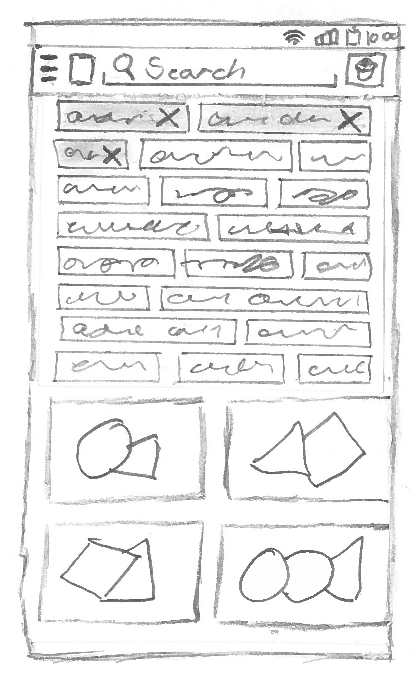
\includegraphics[width=0.7\columnwidth]{../img/prototypes/ingredient_search_tile.pdf}
\caption{Ingredient search with tile selection\label{fig:ingreani}}
\end{minipage}
\hspace{0.5cm}
\begin{minipage}[b]{0.5\columnwidth}
\centering
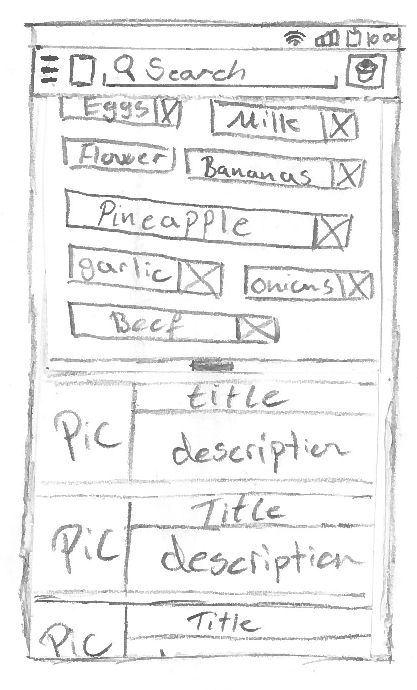
\includegraphics[width=0.72\columnwidth]{../img/prototypes/recipe_browse2.pdf}
\caption{Recipe browsing with selected ingredients \label{fig:recipeword}}
\end{minipage}
\end{figure}

The vision for the project is to digitalise a cookbook so users easily can search for recipes and find instruction for dishes. 

\autoref{fig:ingreani} shows the ingredient search page. The idea with the design is so the user can quickly navigate to the ingredient they want with a few presses. This makes it easier to find ingredients with one hand, which is common when you are out shopping and you have a basket in one hand. The user starts searching by clicking the search field at the top, which is indicated with the ``Magnifying glass''. When the user starts searching, a word cloud appear. The functionality of the word cloud is to suggest ingredients to the user based on the ingredients they already put in. This should help the user to quickly add the ingredients they want. 

The problem with this design is if the user prefers to search by text, or perhaps it is too hard for the user to figure out what category the item they are looking for belongs to. Therefore it would be ideal to also have a way for the user to type in their recipes using a keyboard and text and some sort of autocomplete to help the user.

\autoref{fig:recipeword} shows the recipe browse page. There the user has an overview of the recipes that matches the user's ingredients. The user can still see the ingredients they put in which allows them to quickly add or remove ingredients from their search. However, the space is quite limited so the user cannot see many recipes at a time. This could be changed by removing the ingredient view when browsing the recipes and then the user would have to click the search field again in order to add or remove ingredients, or the ingredients could be hidden when you scroll up and down, allowing the user a full view of recipes when scrolling but see their inputted ingredients when not.

\subsection*{Story, Alice}

Alice is at home, earlier she found a Lasagne recipe and she has already bought all the ingredients for it. She opens the application, goes to the favourites page, and opens her previously favourited recipe for Lasagne. In the recipe she scrolls down to the instructions and follows these in order to make her dinner.


\begin{figure}[H]
\begin{minipage}[b]{0.5\columnwidth}
\centering
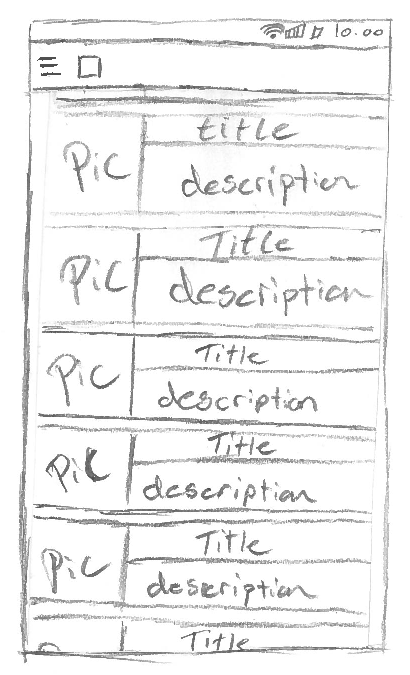
\includegraphics[width=0.7\columnwidth]{../img/prototypes/favorites.pdf}
\caption{The layout for favourites\label{fig:favourite}}
\end{minipage}
\hspace{0.5cm}
\begin{minipage}[b]{0.5\columnwidth}
\centering
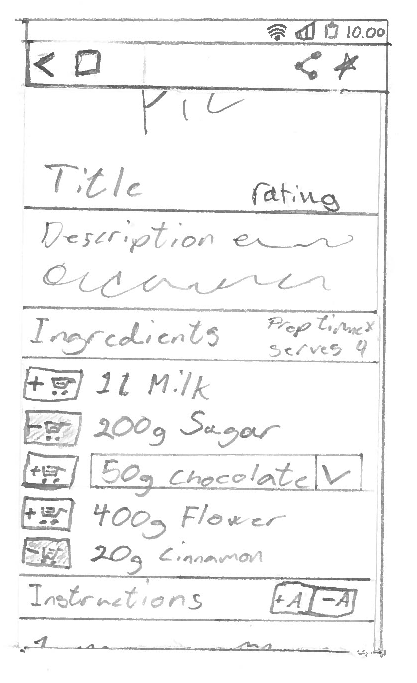
\includegraphics[width=0.735\columnwidth]{../img/prototypes/recipe_new.pdf}
\caption{Redesigned recipe layout\label{fig:recipenew}}
\end{minipage}
\end{figure}

The user must be able to bookmark recipes in order to find them fast when they have to use them.

\autoref{fig:favourite} shows the favourite list. The favourite list is a list of recipes, which allows the user to quickly navigate between them. The simply press the recipe they want to look at and they are taken to it. The recipe page can be seen on \autoref{fig:recipenew}. 

The layout for favourites is very simple and it looks like the page where you browse recipes after having searched. The similar look can be a good thing, since the user is familiar with the layout so they know what happens when you click a recipe.

The recipe consists of a picture of the dish, a title and a rating. Under the picture there is a short description. Then a list of ingredients and the list of instruction the user has to follow. If any of the ingredients can be exchanged with something else, there is a box around it and a drop down menu where you can choose one of the other ingredients.

All the information the user get on the recipe page might seem cluttered for the user until they learn to use the system. Perhaps the first time the user uses the application a small introduction could be shown, displaying the different functionalities in the application.

\section*{Novelty Scale}
\begin{description}[noitemsep]
\item[Level 1] Routine design problems solved by methods well known within the specialty - usually 
no invention needed.
\item[Level 2] Minor improvements to an existing system using methods known within the industry.
\item[Level 3] Fundamental improvement to an existing system using methods known outside the 
industry.
\item[Level 4] A new generation of a system that entails a new principle for performing the system's 
primary functions - solutions are found more often in science than technology.
\item[Level 5] A rare scientific discovery or pioneering invention of an essentially new system.
\end{description}

\begin{figure}[H]
\centering
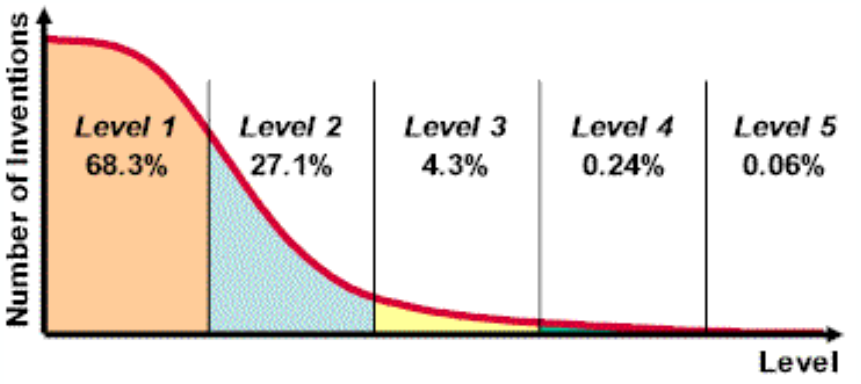
\includegraphics[width=0.7\columnwidth]{Selection_006.png}
\caption{The novelty scale\label{fig:novelty}}
\end{figure}

Based on the nature of our project we have determined that the application is level 2 on the novelty scale. Looking at existing solutions we do not invent any new methods or systems, but we improve on both design and the search algorithm. We do not provide the industry with anything new or innovative, but we make improvements on existing solutions beyond design issues.



%%% Local Variables: 
%%% mode: latex
%%% TeX-master: t
%%% End: 


\section*{Utility forms}

\begin{description}
\item[Computing infrastructural] The product is an application which does not provide any infrastructure to any other technology. We only provide an internal API from the application to the server which contains the recipes.
\item[Technology enabling] Our application does not enable any other technology.
\item[User service] This is the primary focus of the project. There already exists a lot of different solutions and alternatives, but we will extend the existing search functionality, improve the usability of it, and improve the overall quality of the service.
\item[Business change enabling] The users of the application are consumers and not businesses.
\item[Interaction communication] We plan to allow users to create their own recipes and also share them. Users should also be able to rate recipes and also comment on them. Users can also privately share shopping lists with friends or relatives.
\item[Entertainment] The application provides entertainment in the form of food which can be enjoyed with the company of others. Users can discover recipes as well as cultural dishes and share their own.
\end{description}

\section*{Process}

We use the tool called Pivotal Tracker which allows us to create and schedule issues related to the project. For each issue we can see who is working on it and how much estimated work is related to the assignment.

We use low tech prototyping process strategy. We have a few different paper prototypes.

The innovation process strategy we used is "Modifying". We looked at existing solutions and we combined the good parts with our own innovative parts. Particularly we have looked at the different existing solutions and tried to figure our how they work, we picked the one we think is best and have modified it in order to refine and optimize it.

\section*{Innovative process}

We started by brainstorming features, i.e. looking at what features we really wanted to have. Then we looked at existing solutions to see advantages and disadvantages in their solutions. Then we brainstormed features again.

%tools: prototypes?

We conceptualized our project with prototypes. As a result of the prototypes we discovered that some of the initial ideas was not possible and ultimately had to limit some of the user interface functionalities.

\end{document}